\documentclass{exercices}
\usepackage{ae, aeguill, graphicx}
\usepackage{fullpage}
\usepackage{xspace}
\usepackage{color}
\usepackage{amsmath, amssymb}
\usepackage{latexsym}
\usepackage{url}
\usepackage{tikz}
\usetikzlibrary{decorations}
\usetikzlibrary{decorations.fractals}
\usepackage{multicol}
\usepackage{verbatim}

\renewcommand{\|}{\url|}
\begin{document}
\sujet{INF 821: Project - Sudoku generator}

In this project you will design and implement a Sudoku computer game.
Your application will generate valid Sudoku grids, and provide a GUI
(Graphical User Interface) that allows the user to play the generated 
grid. 

\section{Sudoku rules}

Sudoku is played on a $9\times 9$ grid. The grid can be divided into 
nine columns, nine rows and nine blocks of $3\times 3$ cells.
\begin{figure}[h]
\begin{center}
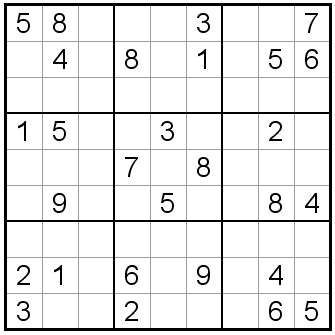
\includegraphics[width=150px]{sudoku_grid}
\end{center}
\caption{A sudoku grid}
\end{figure}

Before the game starts some of the cells have a number from 1 to 9.
To solve the grid the player must fill all the remaining cells using 
numbers from 1 to 9, in a way that satisfies the \emph{Sudoku rule}: 
all the numbers inside a particular row, column or block must be different.

\section{Requirements}

\subsection{Essential requirements}

\begin{itemize}
\item Your application will generate Sudoku grids that have one and only one
  solution.
\item The player will solve the generated grids using a GUI.
\item The GUI will show a Sudoku grid, the player must be able to set or unset
  the value of all the initially empty cells.
\item When the player finishes completing a grid:
  \begin{itemize}
    \item If the grid is correct (satisfies the \emph{Sudoku rule}), a win message is displayed and a new grid is
      proposed.
    \item If the grid is incorrect (does not satisfy the \emph{Sudoku rule}),
      the conflicting cells are highlighted, the player may pursue the game and
      correct his mistake.
  \end{itemize}
\end{itemize}

\subsection{Bonus requirements}
These bonus requirements are hard to implement and are not mandatory (only for
extra credit). Do \emph{not} start working on them before implementing all the essential requirements. 

\begin{itemize}
  \item The user may ask for a grid among three difficulty levels (``easy'',
    ``intermediate'', ``hard'').
  \item The level will indicate how hard it is for a \emph{human} to solve the
    generated grid. 
  \item You must devise a method to gauge the difficulty for a \emph{human} to
    solve a particular grid. A possibility is to design a resolution algorithm 
    that try to play as a human player would (no guessing, 
    only logic inference rules). The complexity and number of rules needed to 
    solve a grid, will give you a good guess of the ``human'' difficulty of the grid.
\end{itemize}
\end{document}
